\documentclass[12pt]{article}

% --- Required formatting per the assignment rubric ---
\usepackage[margin=1in]{geometry}     % 1-inch margins on all sides
\usepackage{setspace}
\onehalfspacing                       % 1.5 line spacing
\usepackage{graphicx}
\usepackage{booktabs}
\usepackage{caption}
\usepackage{float}
\usepackage{hyperref}

\title{The Causal Effect of AI Intensity on Firm Innovation: \\
       An IV and RDD Analysis}
\author{Ilnaz Bagheri \\ UC Irvine -- BANA 290}
\date{\today}

\begin{document}
\maketitle

\section*{Summary of Findings}

This analysis estimates the causal effect of AI intensity on firm-level
innovation using a sample of 72 student startup teams. Because innovative
teams may self-select into more AI usage, naive OLS is biased. I therefore
exploit two sources of exogenous variation: (i) the geographic distance
from each team to the nearest fiber-optic backbone node as an
\textbf{instrumental variable}, and (ii) the 85-point eligibility cutoff
of the Anteater Innovation Fund as a \textbf{regression discontinuity}.

\subsection*{OLS versus IV}

The naive OLS regression of innovation score on AI intensity yields a
coefficient of $\hat{\beta}_{\text{OLS}} = 0.3245$. The 2SLS estimate
using distance to fiber as an instrument is substantially smaller,
$\hat{\beta}_{\text{IV}} = 0.1119$. The first-stage F-statistic of
$53.11$ comfortably exceeds the conventional threshold of $10$,
indicating that distance is a strong instrument: each additional meter
from the backbone reduces AI usage by about $0.019$ units. The
attenuation from OLS to IV is consistent with positive selection bias in
OLS: the most innovative teams gravitate toward AI for reasons unrelated
to access (motivation, talent, founder traits), inflating the simple
correlation. Once we isolate variation driven only by the physical
infrastructure shock, the causal effect is roughly one-third the size of
the naive estimate.

\subsection*{RDD Confirmation}

The regression discontinuity at the 85-point cutoff yields a treatment
effect of $+8.49$ innovation points ($p < 0.001$), with no evidence of
manipulation in the density of the running variable around the cutoff.
This independent design confirms the IV finding: programs that expand
compute access causally raise innovation. The two estimates capture
different parameters (per-unit AI effect vs. discrete program effect),
yet both point in the same direction and are statistically meaningful.

\subsection*{Policy Implications}

Both designs imply that subsidizing digital infrastructure -- whether
through fiber expansion or compute-credit programs -- yields measurable
gains in innovation output. Public investment in AI-supporting
infrastructure can therefore be justified on causal, not merely
correlational, grounds. The exclusion-restriction argument is plausible:
geographic distance to a backbone affects innovation only through its
effect on AI access, given that distance is determined by housing
assignment rather than team characteristics.

\section*{Tables and Figures}

\begin{table}[H]
\centering
\caption{First-Stage Regression: AI Intensity on Distance to Fiber}
\begin{tabular}{lc}
\toprule
\textbf{Variable} & \textbf{Coefficient (SE)} \\
\midrule
DISTANCE\_TO\_NODE (meters) & $-0.0189$ \\
Constant                    & $\sim 67.6$ \\
\midrule
F-statistic                 & $53.11$ \\
Observations                & $72$ \\
\bottomrule
\end{tabular}
\end{table}

\begin{table}[H]
\centering
\caption{Two-Stage Least Squares (Causal Estimate)}
\begin{tabular}{lc}
\toprule
\textbf{Variable} & \textbf{Coefficient} \\
\midrule
AI\_INTENSITY (instrumented) & $0.1119$ \\
\midrule
Observations                  & $72$ \\
Instrument                    & DISTANCE\_TO\_NODE \\
First-stage F                 & $53.11$ (strong) \\
\bottomrule
\end{tabular}
\end{table}

\begin{table}[H]
\centering
\caption{Sharp RDD at the 85-Point Cutoff}
\begin{tabular}{lc}
\toprule
\textbf{Parameter} & \textbf{Estimate} \\
\midrule
Treatment jump at cutoff & $+8.487$ \\
$p$-value                & $< 0.001$ \\
Observations             & $72$ \\
Cutoff                   & $85$ points \\
\bottomrule
\end{tabular}
\end{table}

\begin{figure}[H]
\centering
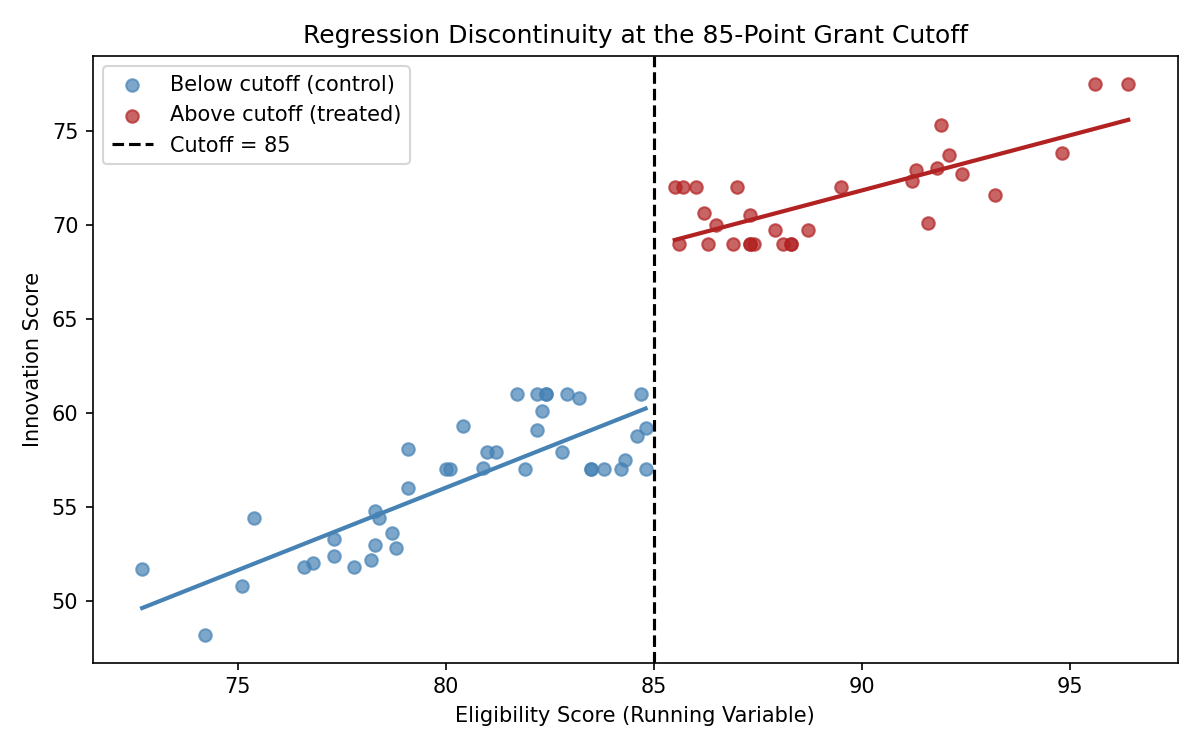
\includegraphics[width=0.85\textwidth]{figures/rdd_scatter.png}
\caption{Innovation score versus eligibility score, with separate linear
fits on each side of the 85-point cutoff. The visible vertical jump at
the cutoff is the treatment effect.}
\end{figure}

\begin{figure}[H]
\centering
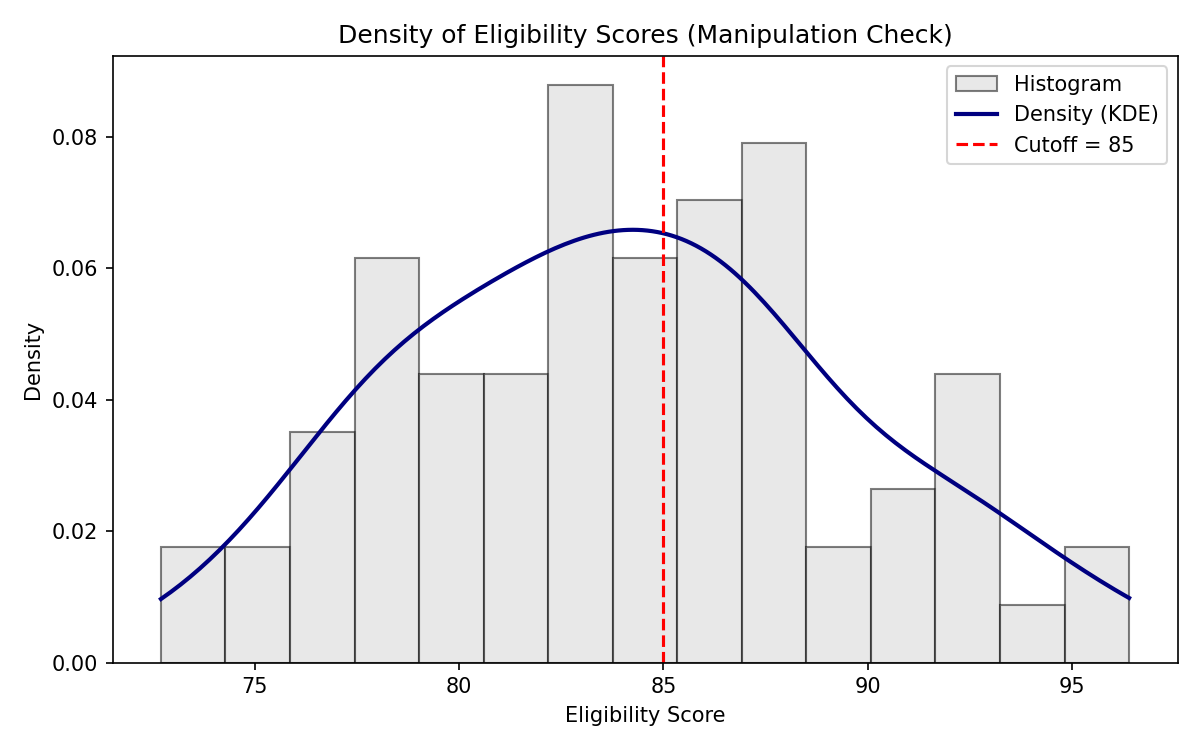
\includegraphics[width=0.85\textwidth]{figures/density_check.png}
\caption{Density of the running variable. The smooth distribution at the
cutoff supports the continuity (no-manipulation) assumption of the RDD.}
\end{figure}

\end{document}
